\documentclass[12pt,a4paper,austrian]{article}
\usepackage{graphicx}
\usepackage[austrian, english]{babel}
\usepackage[utf8]{inputenc}
%\usepackage{listings}
\usepackage{multirow}
\usepackage{epstopdf}
\usepackage{amsmath}
\usepackage{amssymb} % fuer Mengen \N, Q, C, R
\graphicspath{{./fig/}}


%% Satzspiegel
\setlength{\hoffset}{-1in} \setlength{\textwidth}{18cm}
\setlength{\oddsidemargin}{1.5cm}
\setlength{\evensidemargin}{1.5cm}
\setlength{\marginparsep}{0.7em}
\setlength{\marginparwidth}{0.5cm}

\setlength{\voffset}{-1.9in}
\setlength{\headheight}{12pt}
\setlength{\topmargin}{2.6cm}
   \addtolength{\topmargin}{-\headheight}
\setlength{\headsep}{3.5cm}
   \addtolength{\headsep}{-\topmargin}
   \addtolength{\headsep}{-\headheight}
\setlength{\textheight}{27cm}

%% How should floats be treated?
\setlength{\floatsep}{12 pt plus 0 pt minus 8 pt}
\setlength{\textfloatsep}{12 pt plus 0pt minus 8 pt}
\setlength{\intextsep}{12 pt plus 0pt minus 8 pt}

\tolerance2000
\emergencystretch20pt

%% Text appearence
% English text
\newcommand{\eg}[1]%
  {\selectlanguage{english}\textit{#1}\selectlanguage{austrian}}

\newcommand{\filename}[1]
  {\begin{small}\texttt{#1}\end{small}}

\newcommand\IFT{\unitlength1mm\begin{picture}(10,2) \put (1,1)
{\circle{1.7}} \put(2,1){\line(1,0){5}} \put(8,1)
{\circle*{1.7}}\end{picture}}
\newcommand\FT{\unitlength1mm\begin{picture}(10,2) \put (1,1)
{\circle*{1.7}} \put(2,1){\line(1,0){5}} \put(8,1)
{\circle{1.7}}\end{picture}}

% A box for multiple choice problems
\newcommand{\choicebox}{\fbox{\rule{0pt}{0.5ex}\rule{0.5ex}{0pt}}}

\newenvironment{wahrfalsch}%
  {\bigskip\par\noindent\makebox[1cm][c]{richtig}\hspace{3mm}\makebox[1cm][c]{falsch}
   \begin{list}%
   {\makebox[1cm][c]{\choicebox}\hspace{3mm}\makebox[1cm][c]{\choicebox}}%
   {\setlength{\labelwidth}{2.31 cm}\setlength{\labelsep}{3mm}
    \setlength{\leftmargin}{2.61 cm}\setlength{\listparindent}{0pt}
    \setlength{\itemindent}{0pt}}%
  }
  {\end{list}}

\newcounter{theaufgabe}\setcounter{theaufgabe}{1}
\newenvironment{aufgabe}[1]%
  {\bigskip\par\noindent\begin{nopagebreak}
   \textsf{\textbf{\arabic{theaufgabe}.\thinspace Aufgabe}}\quad
      \textsf{\textit{#1}}\\*[1ex]%
\stepcounter{theaufgabe}\hspace{2ex}\end{nopagebreak}}
  {\par\pagebreak[2]}

% Innerhalb der Aufgaben erfolgt die weitere Unterteilung mittels einer
% enumerate Umgebung, die allerdings a), b),... zaehlen soll.
\renewcommand{\labelenumi}{\alph{enumi})}
\renewcommand{\labelenumii}{\arabic{enumii})}

% A box to tick for everything which has to done
\newcommand{\abgabe}{\marginpar{$\Box$}}
% Margin paragraphs on the left side
\reversemarginpar

% Language for listings
%\lstset{language=Vhdl,
%  basicstyle=\small\tt,
 % keywordstyle=\tt\bf,
 % commentstyle=\sl}

% No indention
\setlength{\parindent}{0.0cm}
% Don't number sections
\setcounter{secnumdepth}{0}


%% Beginning of the text

\begin{document}
\selectlanguage{austrian}
\pagestyle{plain}


%===  This is the header section ============================================================
\thispagestyle{empty}
\noindent
\begin{minipage}[b][4cm]{1.0\textwidth}  
\begin{center}
\begin{bf} 
\begin{large} Digital Signal Processing SS 2024 -- 2.~Assignment\end{large} \\
\vspace{0.3cm}
\begin{Large} Discrete Time Signals, Convolution, DTFT  \end{Large} \\
\vspace{0.3cm}
\end{bf}
\begin{large}
Group 22\\
Julian Feichtinger, K12015812\\
Wolfram Laube, K08900915\\
\end{large} 
\end{center}
\end{minipage}

\noindent \rule[0.8em]{\textwidth}{0.12mm}\\[-0.5em]
%=======================================================================================


\begin{aufgabe}{Discrete Time Signals (30\%)}

\begin{enumerate}

\item[(a)]
The following discrete time signals should be plotted in Matlab as indicated in figure \ref{fig:ex1_required_plot_layout}.
The time axis should be labeled with the correct time values and the signals should be plotted using a solid line.
\[
\begin{array}{ll}
x_{1}[n] = -4 \delta[n+3] + 4 \delta[n] - \delta[n-3] + 2 \delta[n-7] & \text{for } -5 \leq n \leq 10 \\
x_{2}[n] = e^{-0.31 n} & \text{for } -5 \leq n \leq 10 \\
x_{3}[n] = 3 \sin \left(2 \pi \frac{3.5}{64} n\right) & \text{for } 0 \leq n \leq 256 \\
x_{4}[n] = -\cos \left(\frac{9}{64} n\right) & \text{for } 0 \leq n \leq 256
\end{array}
\]
To indicate the discrete time nature of the signals, the \texttt{stem} command should be used, unless the signal length becomes too long, in which case the \texttt{plot} command should be used instead.
Choose the ideal way to plot the signals.
Extend the Matlab script \texttt{dsp\_A2\_1.m}.
Useful commands are \texttt{figure}, \texttt{stem}, \texttt{plot}, \texttt{subplot}, \texttt{xlabel}, \texttt{ylabel}, \texttt{title}, \texttt{legend}, \texttt{hold on}, \texttt{grid on}, \texttt{pi}.
You can use the provided function \texttt{impseq}.

\begin{figure}[h]
\centering
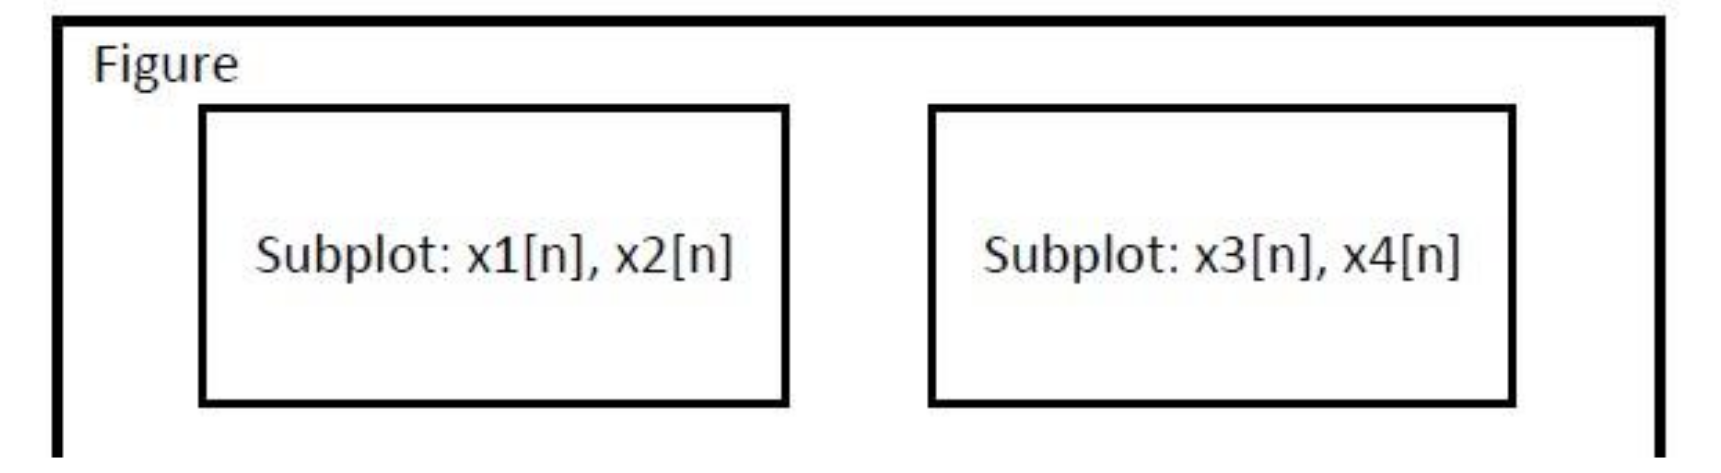
\includegraphics[width=\textwidth]{fig/ex1_required_plot_layout}
\caption{Required arrangement of plots}
\label{fig:ex1_required_plot_layout}
\end{figure}

\item[(b)]
What is the normalized angular frequency $\Omega$ for $x_{3}[n]$ and $x_{4}[n]$?

\item[(c)]
Are the signals $x_{3}[n]$ and $x_{4}[n]$ periodic? If yes, what is their fundamental period?

\item[(d)]
Write the Matlab function \texttt{custom\_power} which calculates the mean power of a discrete time periodic signal according to
\[ P = \frac{1}{N} \sum_{n=0}^{N-1} |x[n]|^2 \]
Pass exactly one signal period to this function to calculate the powers of all periodic signals in (a).

\item[(e)]
Now assume that all signals in (a) are zero outside the plot range (e.g., $x_{2}[11] = 0$).

Write a function \texttt{energy} which calculates the signal energy according to
\[ W = \sum_{n=-\infty}^\infty |x[n]|^2 \]
Determine the energies for all these time-limited signals $x_{1}[n]$ to $x_{4}[n]$.

\item[(f)]
Collect all the signal powers of (d) and signal energies of (e) in a single table in your protocol.
\end{enumerate}

\hrule
\begin{enumerate}
%! Author = wolfram_e_laube
%! Date = 17.04.24

\item[(a)]
The discrete time signals are plotted with the appropriate commands to display the nature of the signals.
For the signals $x_{1}[n]$ and $x_{2}[n]$, the stem command is used to emphasize their discrete nature,
and for the longer signals $x_{3}[n]$ and $x_{4}[n]$, the plot command is utilized.

\begin{verbatim}
% Define the sample ranges
n1 = -5:10;
n2 = 0:256;

% Define the signals
x1 = -4 * (n1 == -3) + 4 * (n1 == 0) - (n1 == 3) + 2 * (n1 == 7);
x2 = exp(-0.31 * n1);
x3 = 3 * sin(2 * pi * 3.5/64 * n2);
x4 = -cos(9/64 * n2);

% Plot the signals
figure;
subplot(2,2,1);
stem(n1, x1, 'filled');
title('Signal x1[n]');

subplot(2,2,2);
stem(n1, x2, 'filled');
title('Signal x2[n]');

subplot(2,2,3);
plot(n2, x3);
title('Signal x3[n]');

subplot(2,2,4);
plot(n2, x4);
title('Signal x4[n]');
\end{verbatim}

%! Author = wolfram_e_laube
%! Date = 17.04.24

\item[(b)]
The normalized angular frequency $\Omega$ is calculated as follows:
- For $x_{3}[n] = 3 \sin\left(2 \pi \frac{3.5}{64} n\right)$, $\Omega = \frac{2 \pi \times 3.5}{64}$.
- For $x_{4}[n] = -\cos\left(\frac{9}{64} n\right)$, $\Omega = \frac{2 \pi \times 9}{64}$.

%! Author = wolfram_e_laube
%! Date = 17.04.24

\item[(c)]
Both signals $x_{3}[n]$ and $x_{4}[n]$ are periodic with fundamental periods calculated by $N = \frac{1}{f}$:
- For $x_{3}[n]$, $f = \frac{3.5}{64}$, so $N = \frac{64}{3.5}$.
- For $x_{4}[n]$, $f = \frac{9}{64}$, so $N = \frac{64}{9}$.

%! Author = wolfram_e_laube
%! Date = 17.04.24

\item[(d)]
This function calculates the mean power of a discrete time periodic signal over a specified number of samples $N$,
which is typically one period of the signal.
The function is defined to take two arguments: the signal array and its period.

\begin{verbatim}
def custom_power(x, N):
    """
    Calculates the mean power of a discrete time periodic signal over N samples.
    """
    return np.sum(np.abs(x)**2) / N
\end{verbatim}

To calculate the mean power of a periodic signal \(x_3[n]\) and \(x_4[n]\),
where the periods have been previously defined based on their frequencies,
the function is called with the signal truncated to one period:

\begin{verbatim}
# Python example
power_x3 = custom_power(x3_values[:18], 18)
power_x4 = custom_power(x4_values[:7], 7)
\end{verbatim}

and yields:

\begin{verbatim}
Power x_3: 4.5657532755203984
Power x_4: 0.4949681510722214
\end{verbatim}

This approach ensures that the power calculation reflects the actual energy content per cycle of the periodic signals,
providing an accurate measure crucial for signal analysis tasks.
%! Author = wolfram_e_laube
%! Date = 17.04.24

\item[(e)]
This function calculates the total energy of a signal:

\begin{verbatim}
def energy(x):
    """Calculates the total energy of the signal."""
    return np.sum(np.abs(x)**2)
\end{verbatim}

and yields:
\begin{verbatim}
Energy x_1: 37
Energy x_2: 48.03937311125317
Energy x_3: 1152.0
Energy x_4: 128.99999999999994
\end{verbatim}

%! Author = wolfram_e_laube
%! Date = 17.04.24

\item[(f)]
All signal powers and energies computed in the previous steps are collected into a single table for a comprehensive overview.
This table facilitates comparison and further analysis:

\begin{verbatim}
import pandas as pd

# Create a dictionary with the data
data = {
    'Signal': ['x1', 'x2', 'x3', 'x4'],
    'Energy': [energy_x1, energy_x2, energy_x3, energy_x4],
    'Power': [None, None, power_x3, power_x4]  # None for non-periodic signals
}

# Create and display a DataFrame
df = pd.DataFrame(data)
print(df)
\end{verbatim}

and reads:

\begin{verbatim}
  Signal       Energy     Power
0     x1    37.000000       NaN
1     x2    48.039373       NaN
2     x3  1152.000000  4.565753
3     x4   129.000000  0.494968
\end{verbatim}

This structure enables easy visualization and access to the energy and power data associated with each signal, making it straightforward to draw comparisons and perform subsequent analyses.

\end{enumerate}

\end{aufgabe}

\begin{aufgabe}{Convolution-1 (20\%)}

The signal $x[n]=(3,-1,2,0,1)$ at sample times $n=(0,1,2,3,4)$ is the input to an LTI system with impulse response $h[n]=(2,3,4,1)$ at sample times $n=(0,1,2,3)$.

\begin{enumerate}
\item[(a)]
How long is the output signal $y[n]$?
\item[(b)]
Manually calculate the output signal $y[n]$.
\end{enumerate}
\hrule

\begin{enumerate}
%! Author = wolfram_e_laube
%! Date = 02.04.24

\item [a)]
Given the cosine wave expressed as
$$
x(t) = \hat{X} \cos(2\pi f_0 t),
$$
we aim to prove its Fourier transform pair. Using Euler's formula, $\cos(\theta) = \frac{e^{j\theta} + e^{-j\theta}}{2}$, we can express the cosine function as a sum of complex exponentials:
$$
x(t) = \hat{X} \left( \frac{e^{j2\pi f_0 t} + e^{-j2\pi f_0 t}}{2} \right) = \frac{\hat{X}}{2} e^{j2\pi f_0 t} + \frac{\hat{X}}{2} e^{-j2\pi f_0 t}.
$$

The Fourier transform of a complex exponential function is given by:
$$
e^{j2\pi f_0 t} \leftrightarrow \delta(f-f_0)
$$
and
$$
e^{-j2\pi f_0 t} \leftrightarrow \delta(f+f_0).
$$

Therefore, applying the Fourier transform to $x(t)$, we obtain:
$$
X(f) = \frac{\hat{X}}{2} \delta(f-f_0) + \frac{\hat{X}}{2} \delta(f+f_0),
$$
proving the given Fourier transform pair for the cosine wave.


%! Author = wolfram_e_laube
%! Date = 02.04.24

\item [b)]
Figure~\ref{fig:FourierTransform} shows the Fourier transformed of the above function. \\
\begin{figure}[!ht]
	\centering
	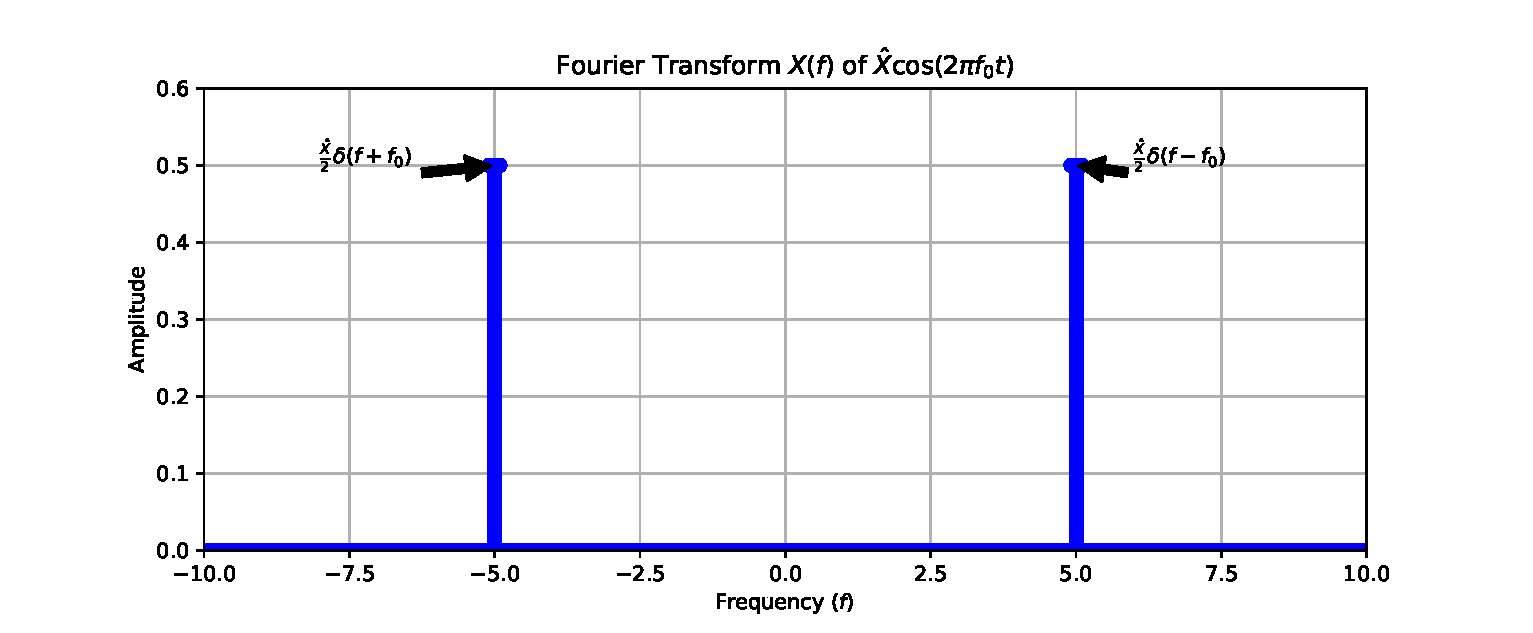
\includegraphics[width=18cm]{ex2_fourier_transformed.eps}
	\vspace{-0.3cm}
	\caption{Fourier Transform.}
	\label{fig:FourierTransform}
	\vspace{-0.1cm}
\end{figure}

\end{enumerate}

\end{aufgabe}

\begin{aufgabe}{Convolution-2 (25\%)}

Consider a Linear Time-Invariant (LTI) system with an impulse response
given by $h[n] = (0.25, 0.5, 0.25)$ at sample indices $n = (0, 1, 2)$.

The input signal is defined as $x[n] = \cos \left(\frac{2 \pi}{20} n\right)$ for $0 \leq n < 50$.

\begin{enumerate}
\item[(a)]
What is the length $L_y$ of the output signal $y[n]$?

\item[(b)]
Implement the convolution operation $y[n] = \sum_{i=0}^{L_{h}-1} h[i] x[n-i]$ in Matlab using two nested for-loops.
The outer for-loop should increment the output index $n$, and the inner for-loop should increment the memory index $i$.
Calculate all $L_y$ output samples of $y[n]$.

\item[(c)]
Plot the signal $y[n]$.

\item[(d)]
Verify the correct implementation of the convolution using the Matlab function \texttt{conv}.
Plot both signals on top of each other, with the directly calculated signal in a solid line style
and the signal obtained via \texttt{conv} in a dashed style.
Provide a legend for your plot.

\end{enumerate}
\hrule

\begin{enumerate}
\item[(a)]
\section*{Exercise 3 Task (a): Frequency Analysis of \(x(t)\)}

\subsection*{Objective}
This task involves identifying all positive frequencies up to 20 kHz in the analog signal \(x(t)\), derived from the discrete-time signal \(x[n]\) through a DAC operating at 8 kHz.

\subsection*{Methodology}
The discrete-time signal \(x[n] = \sqrt{2} \cdot \sin\left(2\pi \frac{1}{8} n\right)\) has a fundamental frequency \(f_0 = 1 \text{kHz}\) because it completes \(\frac{1}{8}\) of a cycle per sample, and the DAC operates at 8 kHz. The analysis focuses on the effects of sampling, which replicates the spectrum around multiples of the sampling frequency, leading to potential frequencies at:
\(f_0\),
\(f_s \pm f_0\),
\(2f_s \pm f_0\)
etc., where \(f_s\) is the sampling frequency (8 kHz).

\subsection*{Results}
The positive frequencies identified in \(x(t)\) and shown in Figure~\ref{fig:exercise3a_frequencies} are:
\begin{itemize}
\item 1 kHz (base frequency)
\item 7 kHz (\(8 \text{ kHz} - 1 \text{ kHz}\))
\item 9 kHz (\(8 \text{ kHz} + 1 \text{ kHz}\))
\item 15 kHz (\(16 \text{ kHz} - 1 \text{ kHz}\))
\item 17 kHz (\(16 \text{ kHz} + 1 \text{ kHz}\))
\end{itemize}

\begin{figure}[h]
    \centering
    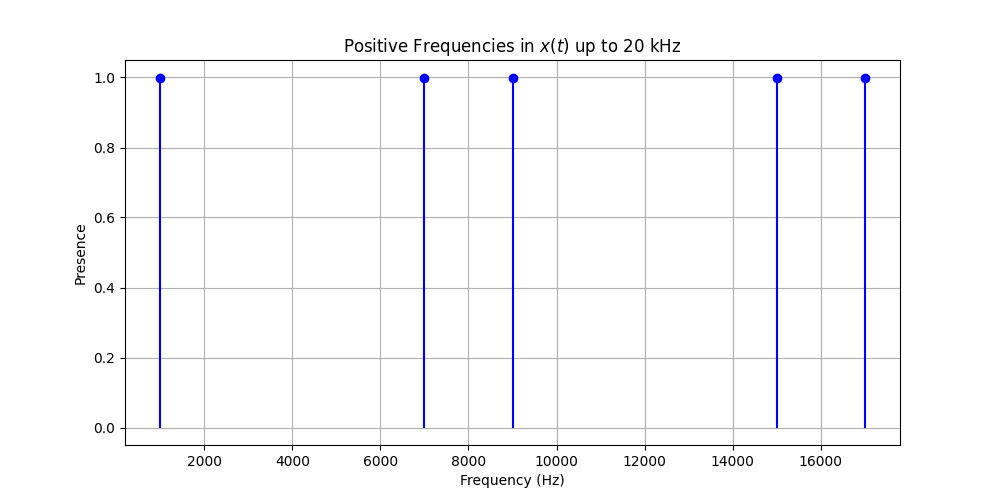
\includegraphics[width=0.8\textwidth]{fig/ex3_task_a_frequencies}
    \caption{Positive frequencies in \(x(t)\) up to 20 kHz}
    \label{fig:exercise3a_frequencies}
\end{figure}

\subsection*{Conclusion}
This detailed frequency analysis underscores the significance of understanding the effects of sampling on the signal's spectrum.
It aids in designing digital systems that effectively manage aliasing and maintain signal fidelity.

\item[(b)]
\section{Pole-Zero Map}

\subsection*{Problem Statement}
Draw a sketch of the pole-zero map.

\subsection*{Theoretical Background}
A pole-zero map is a graphical representation of the locations of the poles and zeros of a transfer function in the complex plane. Poles are typically represented by 'x' marks and zeros by 'o' marks.

\subsection*{Pole-Zero Map}
The given zeros are:
\begin{itemize}
    \item \( N_{1} = -1 \)
    \item \( N_{2} = j \)
    \item \( N_{3} = -j \)
\end{itemize}

The given poles are:
\begin{itemize}
    \item \( P_{1} = 0 \)
    \item \( P_{2} = 0.75 + j0.25 \)
    \item \( P_{3} = 0.75 - j0.25 \)
\end{itemize}

\begin{figure}[h]
    \centering
    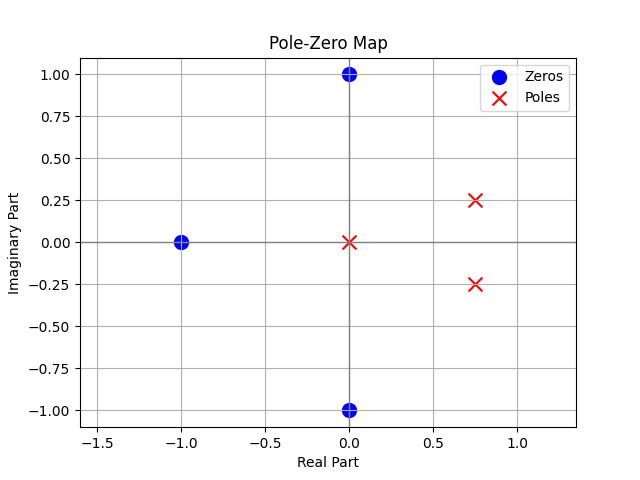
\includegraphics[width=0.8\textwidth]{fig/ex3_b_pole_zero_map.png}
    \caption{Pole-Zero Map}
    \label{fig:ex3_b_pole_zero_map}
\end{figure}

\subsection*{Conclusion}
The pole-zero map shows the locations of the poles and zeros in the complex plane. The zeros are marked with 'o' and the poles with 'x'.

\item[(c)]
\section{Transfer Function with Polynomials of \(z^{-i}\) and \(z^{+i}\)}

\subsection*{Problem Statement}
State the transfer function, first with polynomials of \(z^{-i}\), \(i = 0, 1, 2, 3, \ldots\), and afterwards with polynomials of \(z^{+i}\).

\subsection*{Theoretical Background}
The transfer function \(H(z)\) relates the input \(X(z)\) and output \(Y(z)\) in the z-domain. It can be expressed using polynomials of \(z^{-1}\) (commonly used in digital filter design) and also in terms of \(z\).

\subsection*{Mathematical Derivation}
Given the zeros and poles, we can construct the transfer function.

\subsubsection*{Polynomials of \(z^{-i}\)}
The transfer function \( H(z) \) in terms of \( z^{-1} \):
\[ H(z) = \frac{(z + 1)(z - j)(z + j)}{z(z - (0.75 + j0.25))(z - (0.75 - j0.25))} \]

Simplifying the numerator and the denominator:
\[ (z + 1)(z - j)(z + j) = (z + 1)(z^2 + 1) = z^3 + z^2 + z + 1 \]

The denominator:
\[ z(z - (0.75 + j0.25))(z - (0.75 - j0.25)) = z \left(z^2 - (0.75 + j0.25 + 0.75 - j0.25)z + (0.75^2 - j^2(0.25^2))\right) \]
\[ = z(z^2 - 1.5z + 0.625) = z^3 - 1.5z^2 + 0.625z \]

So, the transfer function is:
\[ H(z) = \frac{z^3 + z^2 + z + 1}{z^3 - 1.5z^2 + 0.625z} \]

Expressing in terms of \( z^{-1} \):
\[ H(z) = \frac{1 + z^{-1} + z^{-2} + z^{-3}}{1 - 1.5z^{-1} + 0.625z^{-2}} \]

\subsubsection*{Polynomials of \(z^{+i}\)}
The transfer function \( H(z) \) in terms of \( z \):
\[ H(z) = \frac{z^3 + z^2 + z + 1}{z^3 - 1.5z^2 + 0.625z} \]

\subsection*{Conclusion}
The transfer function expressed with polynomials of \( z^{-i} \) is:
\[ H(z) = \frac{1 + z^{-1} + z^{-2} + z^{-3}}{1 - 1.5z^{-1} + 0.625z^{-2}} \]

The transfer function expressed with polynomials of \( z^{+i} \) is:
\[ H(z) = \frac{z^3 + z^2 + z + 1}{z^3 - 1.5z^2 + 0.625z} \]

\item[(d)]
\section{Direct-Form I Implementation}

\subsection*{Problem Statement}
Draw the block diagram of a direct-form I implementation of the filter and specify the coefficient values in the block diagram.

\subsection*{Theoretical Background}
A direct-form I implementation of a digital filter uses the difference equation directly to realize the filter structure. It involves using delay elements, multipliers for coefficients, and adders.

Given the transfer function in terms of \( z^{-1} \):
\[ H(z) = \frac{1 + z^{-1} + z^{-2} + z^{-3}}{1 - 1.5z^{-1} + 0.625z^{-2}} \]

The difference equation is:
\[ y[n] = x[n] + x[n-1] + x[n-2] + x[n-3] - 1.5y[n-1] + 0.625y[n-2] \]

\subsection*{Block Diagram}
The block diagram of the direct-form I implementation is shown below:

\begin{figure}[h]
    \centering
    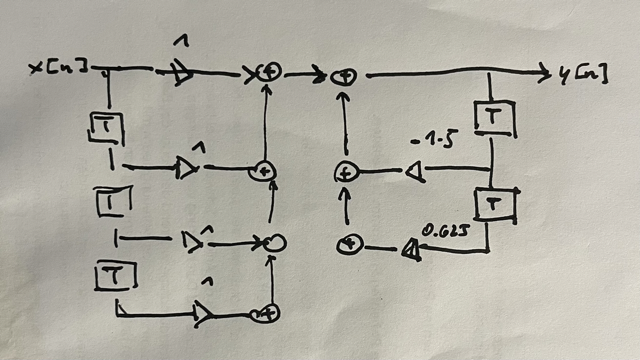
\includegraphics[width=0.8\textwidth]{fig/ex3_d_block_diagram.png}
    \caption{Block Diagram of Direct-Form I Implementation}
    \label{fig:ex3_d_block_diagram}
\end{figure}

\subsection*{Conclusion}
The block diagram of the direct-form I implementation illustrates the structure of the digital filter using delay elements, multipliers, and adders. The coefficient values are specified according to the difference equation.

\end{enumerate}

\end{aufgabe}

\begin{aufgabe}{Discrete Time Fourier Transform (25\%)}
The time discrete sequence $x[n]=(0.8)^{|n|}(u[n+10]-u[n-11])$ should be transformed to the frequency domain
by using the discrete time Fourier transform (DTFT).
As $x[n]$ has finite support (that means it is a sequence of finite length), $X\left(e^{j \Omega}\right)$
can be determined numerically via Matlab (or alternatively Octave, Python).

\begin{enumerate}
\item[(a)]
Create a Matlab function, that is able to calculate the DTFT of a finite sequence.
The function should provide the following interface:

% Interface is described in the attached screenshot.

Try to avoid for loops!
You are still allowed to use for loops, however there will be a small deduction in points for the case you need to use for loops.

\item[(b)]
Plot magnitude and phase response of $X\left(e^{j \Omega}\right)$ for the interval $-\pi \leq \Omega \leq \pi$
within single subplots.
What do you observe for the phase response (hint: you should have a close look at the scaling of the $y$ axis)?

\item[(c)]
Vary the parameter $\Omega$.
What do you observe in the spectrum?
\end{enumerate}

\hrule

\begin{enumerate}
\item[(a)]
\section{Normalized Radian Frequencies and Tolerances}

\subsection*{Problem Statement}
Specify the normalized radian frequencies for the passband \( \Omega_{\text{pass}} \) and the stopband \( \Omega_{\text{stop}} \), the passband tolerance \( \delta_{1} \), and the stopband tolerance \( \delta_{2} \).

Given:
\begin{itemize}
    \item Passband cutoff frequency: \( f_{\text{pass}} = 3.4 \text{kHz} \)
    \item Stopband cutoff frequency: \( f_{\text{stop}} = 4 \text{kHz} \)
    \item Allowed ripple in the passband: \( \pm 5\% \)
    \item Minimum stopband attenuation: \( 45 \text{dB} \)
    \item Sampling frequency: \( f_s = 20 \text{kHz} \)
\end{itemize}

\subsection*{Theoretical Background}
Normalized radian frequencies are calculated using the formula:
\[ \Omega = \frac{2\pi f}{f_s} \]
where \( f \) is the frequency in Hz and \( f_s \) is the sampling frequency in Hz.

Passband tolerance \( \delta_1 \) is the maximum allowed deviation from the desired gain (1) in the passband, given as a percentage.

Stopband tolerance \( \delta_2 \) is derived from the minimum stopband attenuation, given in decibels (dB). It is calculated using the formula:
\[ \delta_2 = 10^{-\frac{A}{20}} \]
where \( A \) is the attenuation in dB.

\subsection*{Mathematical Derivation}

\subsubsection*{Normalized Radian Frequencies}
\begin{itemize}
    \item Passband cutoff frequency:
    \[
    \Omega_{\text{pass}} = \frac{2\pi \times 3400}{20000} = 0.34\pi
    \]
    \item Stopband cutoff frequency:
    \[
    \Omega_{\text{stop}} = \frac{2\pi \times 4000}{20000} = 0.4\pi
    \]
\end{itemize}

\subsubsection*{Passband Tolerance \( \delta_1 \)}
Given \( \pm 5\% \) ripple in the passband, the tolerance is:
\[
\delta_1 = 0.05
\]

\subsubsection*{Stopband Tolerance \( \delta_2 \)}
Given a minimum stopband attenuation of \( 45 \text{dB} \):
\[
\delta_2 = 10^{-\frac{45}{20}} = 10^{-2.25} \approx 0.00562
\]

\subsection*{Conclusion}
The normalized radian frequencies and tolerances for the lowpass filter are:
\begin{itemize}
    \item Passband cutoff frequency \( \Omega_{\text{pass}} = 0.34\pi \)
    \item Stopband cutoff frequency \( \Omega_{\text{stop}} = 0.4\pi \)
    \item Passband tolerance \( \delta_1 = 0.05 \)
    \item Stopband tolerance \( \delta_2 = 0.00562 \)
\end{itemize}

%! Author = wolfram_e_laube
%! Date = 16.04.24

\item[(b)]
The magnitude and phase response of the DTFT is plotted using the following Python code:

\begin{verbatim}
import matplotlib.pyplot as plt
import numpy as np

# Given sequence parameters
n = np.arange(-10, 11)  # Since x[n] is nonzero for n between -10 and 10
x = (0.8)**np.abs(n)

# Frequency vector
w = np.linspace(-np.pi, np.pi, 1000)

# Compute DTFT
X = dtft(x, n, w)

# Plot magnitude and phase response
plt.figure(figsize=(14, 6))

# Magnitude response subplot
plt.subplot(2, 1, 1)
plt.plot(w, np.abs(X))
plt.title('Magnitude Response of $X(e^{j\Omega})$')
plt.xlabel('$\Omega$')
plt.ylabel('|X|')
plt.grid()

# Phase response subplot
plt.subplot(2, 1, 2)
plt.plot(w, np.angle(X))
plt.title('Phase Response of $X(e^{j\Omega})$')
plt.xlabel('$\Omega$')
plt.ylabel('Phase (radians)')
plt.grid()

plt.tight_layout()
plt.show()
\end{verbatim}

This code segment uses Matplotlib to create the plots for the magnitude and phase responses
of the DTFT computed for a discrete sequence.

\begin{figure}[h]
\centering
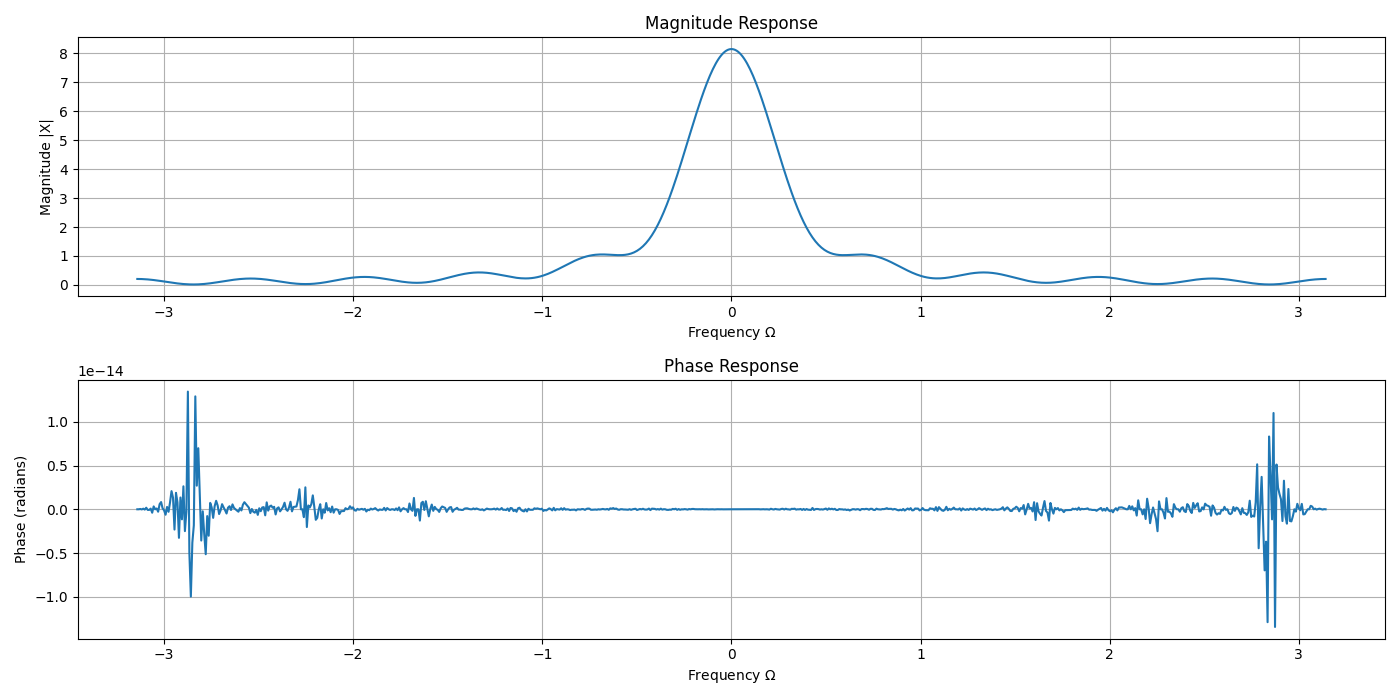
\includegraphics[width=\textwidth]{fig/ex4_b_plot}
\caption{Magnitude and phase of DTFT}
\label{fig:ex4_b_plot}
\end{figure}

\item[(a)]
\section*{Task (a)}

\subsection*{Problem Statement}
% TODO insert problem statement here

\subsection*{Theoretical Background}
% TODO insert theoretical here

\subsection*{Mathematical Derivation}
% TODO insert mathematical derivation here

\subsection*{Python Implementation and Plot}
% TODO insert plot description here
The plot Figure~\ref{fig:ex1_a_plot} below illustrates these this

% TODO insert plot here
\begin{figure}[h]
    \centering
    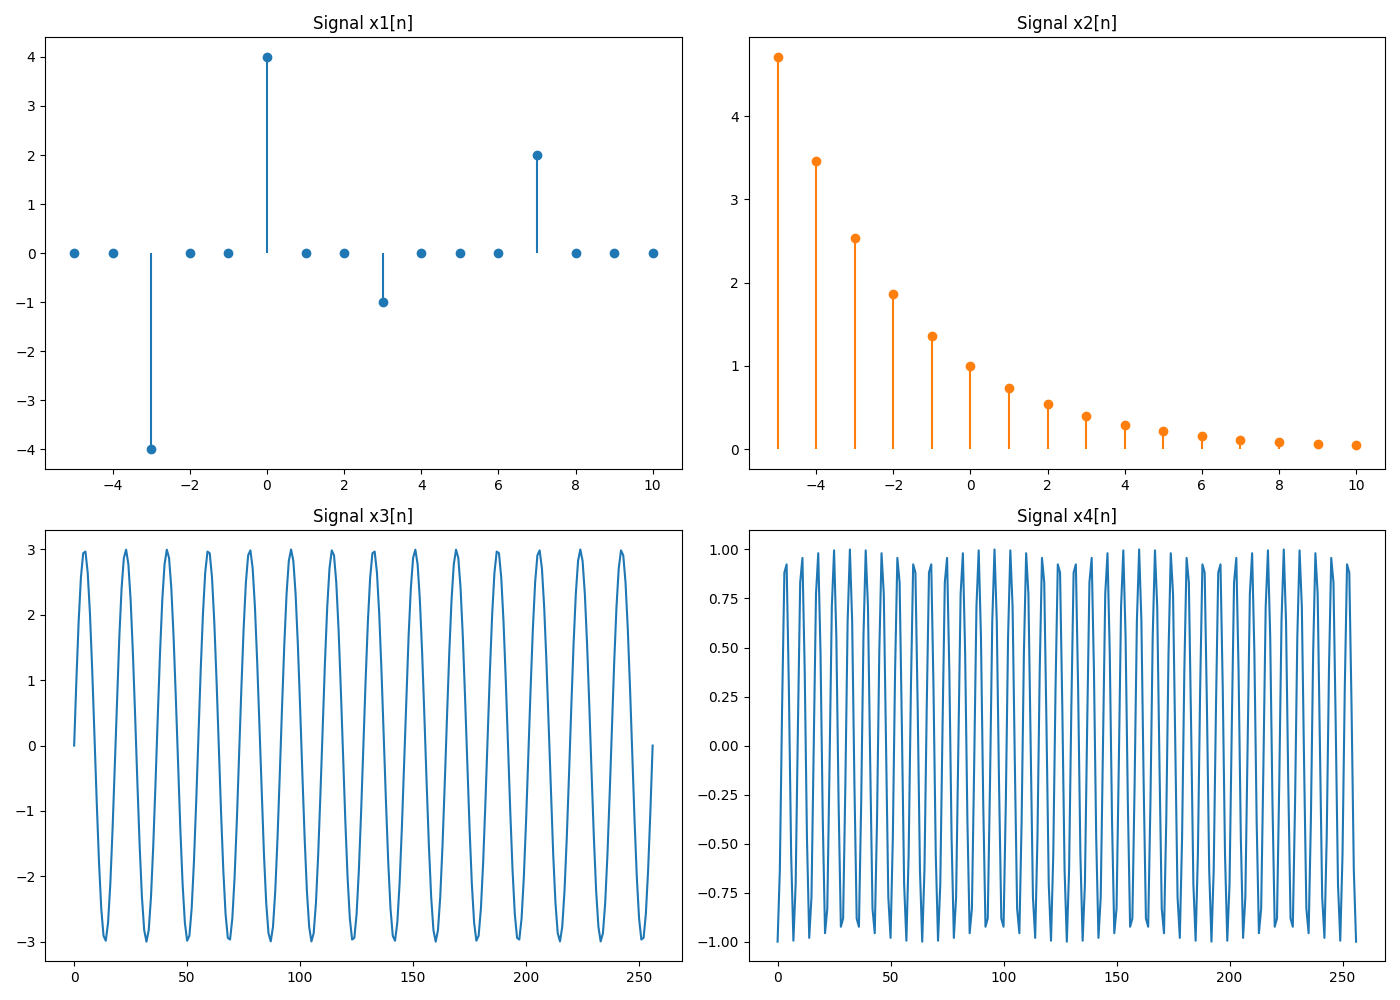
\includegraphics[width=0.8\textwidth]{fig/ex1_a_plot}
    \caption{Exercise 1 Task (a)}
    \label{fig:ex1_a_plot}
\end{figure}

\subsection*{Conclusion}
\end{enumerate}

\end{aufgabe}


\end{document}
